\documentclass{article}
\usepackage[left=2cm,right=2cm,top=3cm,bottom=3cm,letterpaper]{geometry}
\usepackage[spanish]{babel}
\usepackage[utf8]{inputenc}
\usepackage{graphicx}
\usepackage{enumitem}
\usepackage{hyperref}

\title{Prueba y Comparación de Naive Bayes y C4.5}
\author{Juan Carlos López López \and Adolfo Marín Arriaga \and Luis Rodrigo Rojo Morales}
\date{\today\\}
\begin{document}
 \maketitle
 \section{Introducción}
 Para hacer las pruebas de estos algoritmos usamos el conjunto de datos que esta destinado a probar los clasificadores, este se puede obtener en: \href{https://archive.ics.uci.edu/ml/datasets/Adult} {https://archive.ics.uci.edu/ml/datasets/Adult} y en nuestro repositorio se encuentra en: \href{https://github.com/rodrigorojo/ProyectoFinalMineria/blob/master/Entregable3/NaiveBayes/AdultDataSetTest.csv}{/Entregable3/NaiveBayes/AdultDataSetTest.csv}. Dicho conjunto tiene 16,281 registros, los cuales cada uno tiene los mismos atributos que el conjunto de datos original.

 \section{Naive Bayes}
 El script para probar este clasificador se encuentra en \href{https://github.com/rodrigorojo/ProyectoFinalMineria/blob/master/Entregable3/NaiveBayes/TestAdultDataSet.java} {/Entregable3/NaiveBayes/TestAdultDataSet.java} el objetivo de este script es cargar el conjunto de datos prueba, aplicar el clasificador y dar los datos de cuantos clasifico bien y cuantos mal, para así poder hacer la matriz de confusión, la cual queda de la siguiente manera:
 \begin{center}
   \begin{tabular}{|p{2cm}|p{2cm}|p{2cm}|}
     \hline
                  & $>$ 50K & $\leq$ 50K  \\ \hline
      $>$ 50K     & 2920    & 926         \\ \hline
      $\leq$ 50K  & 2107    & 10328        \\ \hline
    \end{tabular}
 \end{center}
 Con esta matriz podemos observar que el clasificador predijo 13248 bien y 3033 mal, a 926 personas le dijimos que iban a ganar $\leq$ 50K pero en realidad ganaron $>$ 50K, mientras que a 2107 personas les dijimos que iban a ganar $>$ 50K pero ganaron $\leq$ 50K.

 El clasificador en general tiene una exactitud del 81.37$\%$, mientras que individualmente predice a los que ganan más de 50K con una exactitud de 75.92$\%$ y a los que ganan menos o 50K con una exactitud de 83.05$\%$
 \section{C4.5}

 El script para probar este clasificador se encuentra en \href{https://github.com/rodrigorojo/ProyectoFinalMineria/blob/master/Entregable3/NaiveBayes/TestAdultDataSet.java} {/Entregable3/C4.5/TestAdultDataSet.java} el objetivo de este script es cargar el conjunto de datos prueba, aplicar el clasificador y dar los datos de cuantos clasifico bien y cuantos mal, para así poder hacer la matriz de confusión, la cual queda de la siguiente manera:
 \begin{center}
   \begin{tabular}{|p{2cm}|p{2cm}|p{2cm}|}
     \hline
                  & $>$ 50K & $\leq$ 50K  \\ \hline
      $>$ 50K     & 2168    & 1648         \\ \hline
      $\leq$ 50K  & 689    & 11746        \\ \hline
    \end{tabular}
 \end{center}
 Con esta matriz podemos observar que el clasificador predijo 13914 bien y 2337 mal, a 1648 personas le dijimos que iban a ganar $\leq$ 50K pero en realidad ganaron $>$ 50K, mientras que a 689 personas les dijimos que iban a ganar $>$ 50K pero ganaron $\leq$ 50K.

 El clasificador en general tiene una exactitud del 85.46$\%$, mientras que individualmente predice a los que ganan más de 50K con una exactitud de 56.81$\%$ y a los que ganan menos o 50K con una exactitud de 94.45$\%$
 \section{Comparación}
 Comparando ambas técnicas de clasificación podemos concluir parcialmente que la técnica de clasificación árboles C4.5 tiene mayor precisión, pero si nos fijamos en cada clase por separado, podemos ver que uno es mejor en diferenciar a los de la calse $\leq$ 50K y otro es mejor en $>$ 50K como se muestra en la siguiente tabla:
\begin{center}
  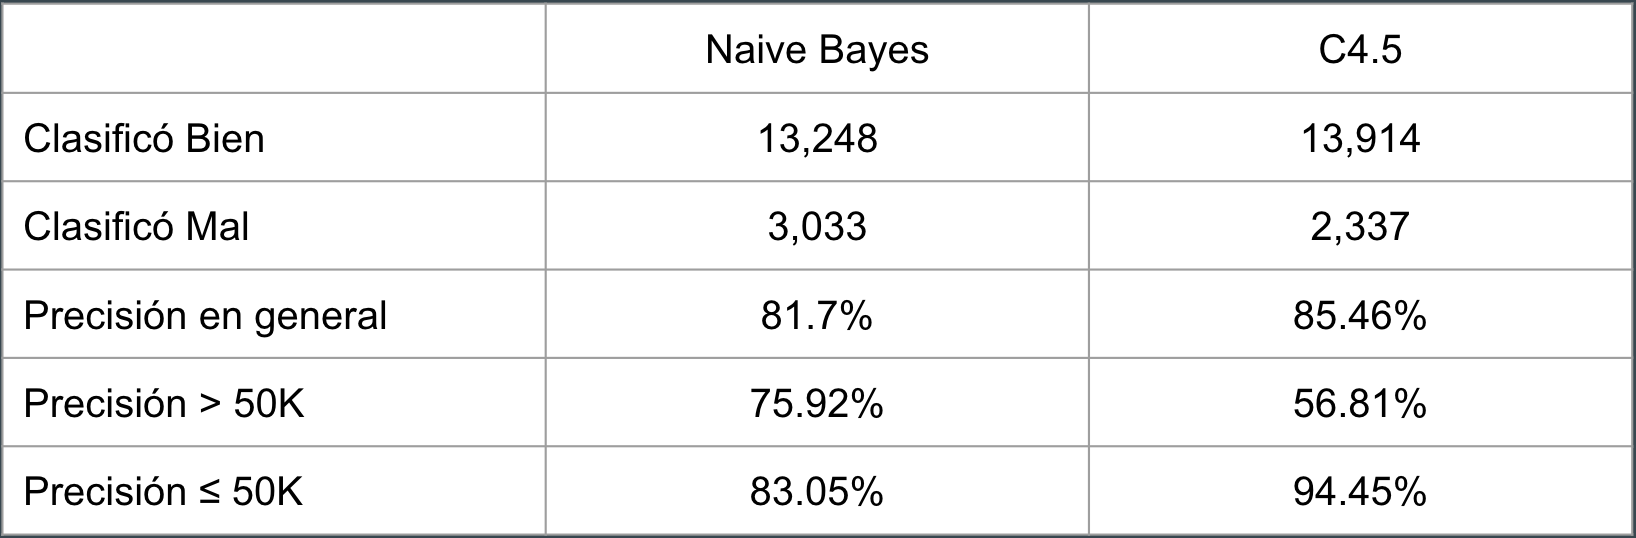
\includegraphics[scale=0.5]{tabla}
\end{center}
El clasificador Naive Bayes es mejor para clasificar a los que ganan más de 50K mientras que C4.5 es mejor para los que ganan $leq$ 50K.
\end{document}
